% !TEX root = main.tex

%This paper is about \emph{relative expressiveness} results for 
%\emph{higher-order process calculi}, core programming languages that 
%integrate name- and process-passing in communications.
%We focus on calculi coupled with \emph{session types} that denote interaction protocols. 
%Expressiveness results allows us to 
%identify
%a \emph{core %process language % concurrency %with session primitives, 
%calculus}
%that encompasses both first- and higher-order session communication.
%Establishing such results 
%in our typed setting 
%is challenging because 
% it entails defining 
% not only a translation 
%relating source and target languages (\emph{encoding}), but also a translation 
%relating their associated session types. 
%We aim at a very particular class of correct encodings: namely \emph{fully abstract} and \emph{type-preserving} encodings.
%Next, we elaborate on our aims,   approach, and contributions.

\emph{Type-preserving compilations} are important in the design of
functional and object-oriented languages: type information has been
used to, e.g., justify code optimizations and reason about programs
(see, e.g.,
\cite{DBLP:journals/toplas/MorrisettWCG99,DBLP:conf/pldi/ShaoA95,DBLP:journals/toplas/LeagueST02}).
A vast literature on 
{\em expressiveness} 
in concurrency theory  
(e.g.,~\cite{Palamidessi03,DBLP:journals/iandc/Gorla10,DBLP:conf/icalp/LanesePSS10})
also studies compilations (or \emph{encodings}):
they are used to transfer reasoning techniques 
from one calculus to another, and to identify 
constructs which may be implemented
using simpler ones. 
%To a large extent, however, this kind of \emph{expressiveness studies} concern only \emph{untyped process languages}.
In this work, we study 
{\em relative expressiveness} 
via \emph{type-preserving encodings} for \HOp, a \emph{higher-order} 
process language that integrates message-passing concurrency with functional features.
We consider source and target calculi coupled with \emph{session types} denoting interaction protocols. 
Building upon untyped frameworks for relative expressiveness
\cite{DBLP:journals/iandc/Gorla10}, 
we propose type preservation as a {new criteria} for \emph{precise encodings}.
We identify \HO, a new core calculus for higher-order session concurrency without
name passing. 
We show that \HO can encode \HOp precisely and efficiently. 
Requiring  
type preservation makes
this encoding far from trivial: our encoding crucially exploits advances on
session type duality~\cite{TGC14,DBLP:journals/corr/abs-1202-2086} and recent
characterisations of typed contextual equivalence \cite{characteristic_bis}.
We develop a full hierarchy of variants of \HOp based on 
precise encodings (see \figref{fig:express}):
our encodings are
type-preserving and fully abstract, up to typed
behavioural equalities. 

\begin{figure}[t]
\centering
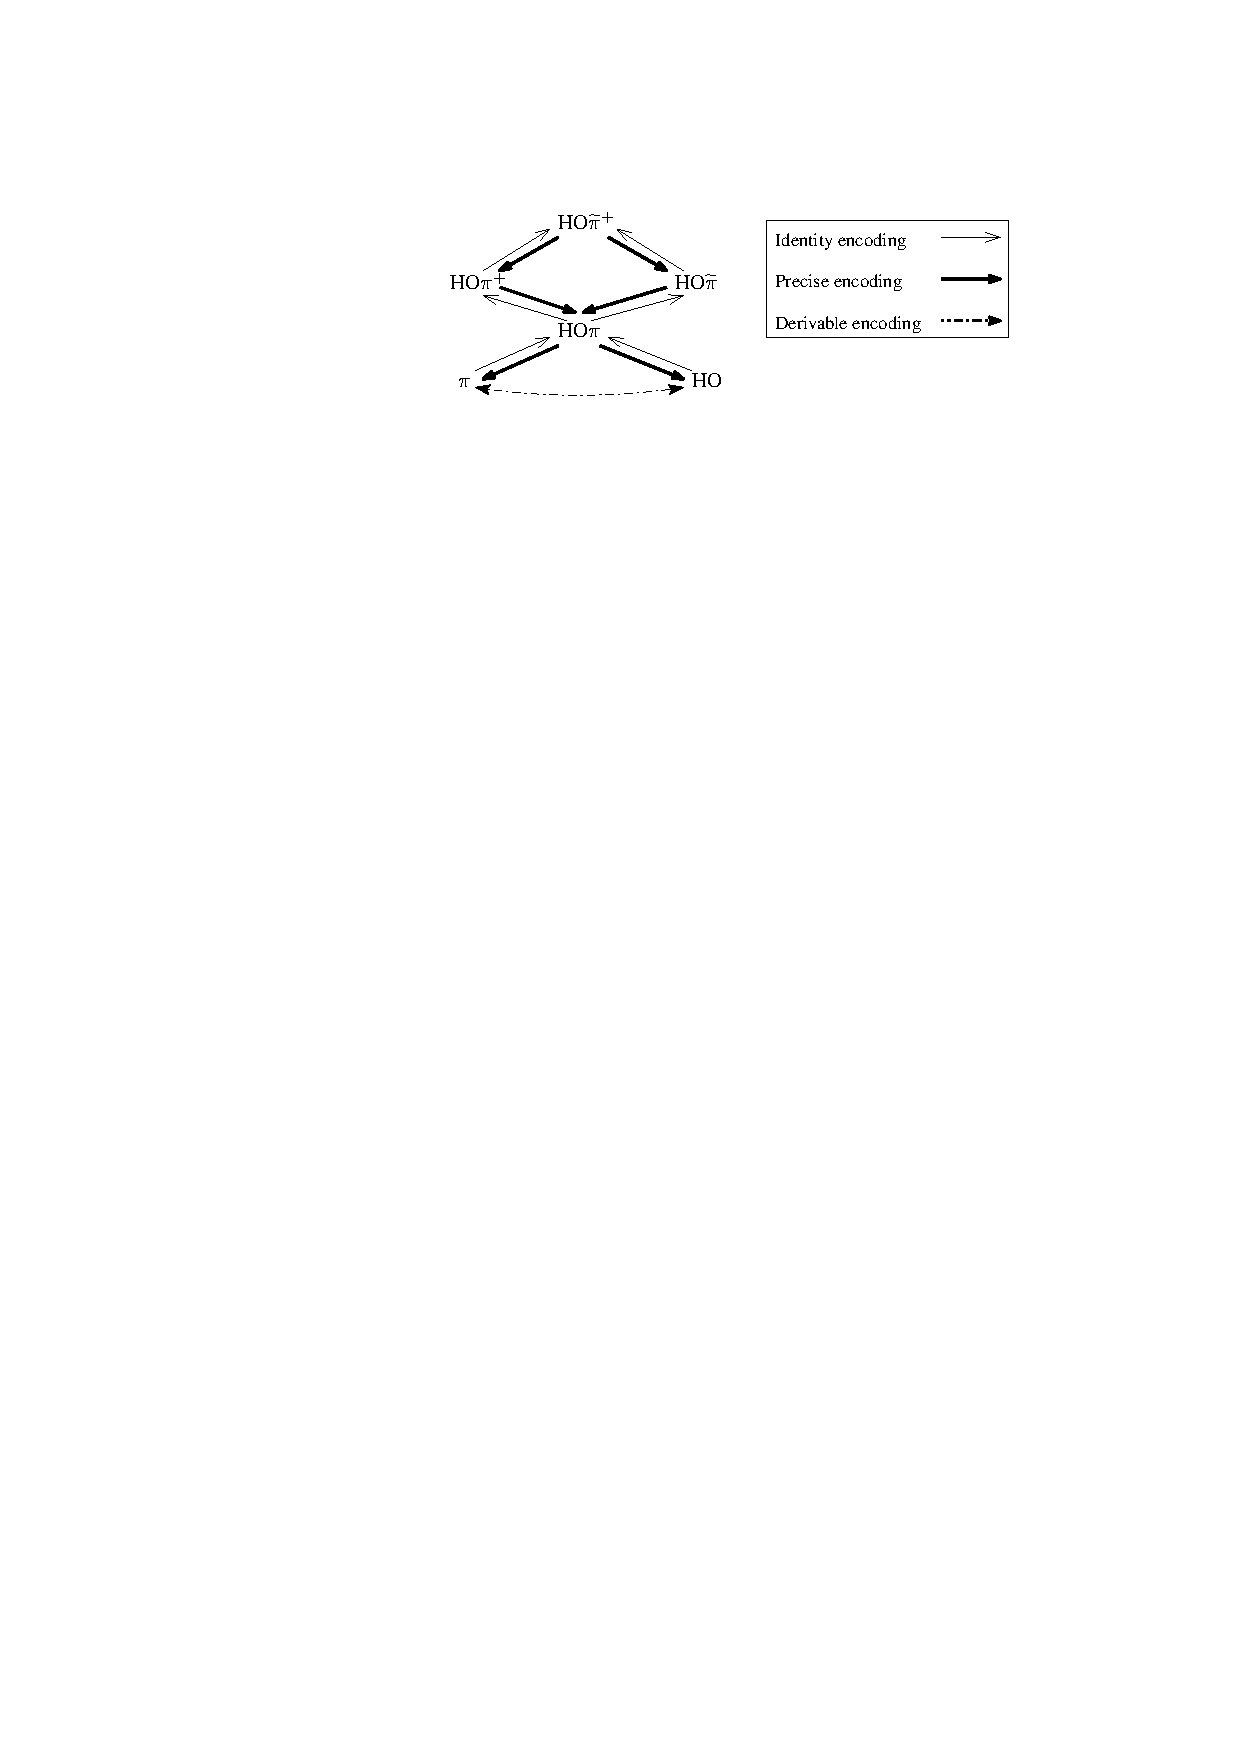
\includegraphics[scale=1]{diag.pdf}

	\caption{Encodability in Higher-Order Sessions. 
	Precise encodings are defined in \defref{def:goodenc}.
	\label{fig:express}}
\vspace{-5mm}
\Hlinefig
\end{figure}

\jparagraph{Context}
In \emph{session-based concurrency}, interactions are organized into \emph{sessions}, basic communication units.
Interaction patterns can then be abstracted as expressive \emph{session types}~\cite{honda.vasconcelos.kubo:language-primitives}, against which  specifications may be checked. 
%These patterns are defined as %(possibly recursive) 
%sequences of communication actions: % (send/receive a value, offer/select a behavior).
%For instance, 
%session type $T_1 = \btinp{\mathsf{str}} \btout{\mathsf{int}}  \tinact$ may be intuitively read as: receive (?) a value of type $\mathsf{str}$,then output (!) a value of type $\mathsf{int}$, finally close the protocol.
Session type $\btinp{U} S$ (resp.  $\btout{U} S$)
describes a protocol that first receives (resp. sends) a value of type $U$ and then continues as protocol $S$.
Also, given an index set $I$, types $\btbra{l_i:S_i}_{i \in I}$ 
and $\btsel{l_i:S_i}_{i \in I}$ 
define %, respectively,
%a branching and selection constructs for  
 a labeled choice mechanism; types 
$\trec{t}{S}$ 
and 
$\tinact$ denote recursive and completed protocols, respectively.
%describes a protocol that offers
%(resp. ) 
%Type $\tinact$ denotes the completed protocol.
In the (first-order) $\pi$-calculus~\cite{MilnerR:calmp1}, 
session types describe the intended interactive behavior of the names/channels in a process.
%names/channels are endowed with session types (such as $T_1$) representing their intended interactive behavior.

Session-based concurrency has also been casted in {higher-order} process
calculi which, by combining features from the $\lambda$-calculus and the $\pi$-calculus, 
enable the exchange of values 
that may contain processes~\cite{tlca07,DBLP:journals/jfp/GayV10}. 
%Higher-order calculi with sessions 
%naturally bridges concurrent and functional computation, 
%and enable the specification of protocols involving \emph{code mobility}, 
%commonplace in practice.
%The \HOp calculus enables 
%the specification of protocols involving \emph{code mobility}, 
%and includes
%Higher-order calculi with sessions 
The higher-order calculus with sessions studied here, denoted \HOp,
can specify protocols involving \emph{code mobility}: it includes
%equiped ping with 
constructs for 
synchronisation along shared names, 
session communication (value passing, labelled choice) along linear names,
recursion, 
 (first-order) abstractions 
 and applications.
 That is, 
 values in communications include names but also (first-order) abstractions---functions from name identifiers to processes. 
 %(In contrast, higher-order abstractions---functions from processes to processes---are disallowed.)
 (In contrast, we rule out higher-order abstractions---functions from processes to processes.)
Abstractions can be linear or shared; their types are  denoted $\lhot{C}$ and $\shot{C}$, respectively ($C$ 
%is a first-order type $C$ (say, a session name).
denotes a name). In \HOp we may have processes with a 
session type such as, e.g.,
%$T_2 = \btbra{upload:\btinp{\lhot{\mathsf{int}}}\tinact ~ , ~ sha:\btinp{\shot{\mathsf{int}}}\tinact}_{}$
$$S = \btbra{up:\btinp{\lhot{C}}\btout{\mathsf{ok}}\tinact ~ , ~ down:\btout{\shot{C}}\btout{\mathsf{ok}}\tinact ~ , ~quit:\btout{\mathsf{bye}}\tinact}_{}$$
that abstracts a server that offers different behaviors to clients: 
%  clients to select among distinct  behaviors: %namely, 
  to \emph{upload} a linear function, % (to be received by the server), 
  to \emph{download} a shared function, % (to be sent by the server),
   or to \emph{quit} the protocol. Subsequently, 
  the server sends a message ($\mathsf{ok}$ or $\mathsf{bye}$) before closing the session.


%\jparagraph{The Problem}
%%Roughly speaking, 
%  \HOp %, a higher-order process language that 
%extends Sangiorgi's higher-order $\pi$-calculus~\cite{SangiorgiD:expmpa} with session primitives.
%To be precise, %More precisely, 
%\HOp
%includes
%constructs for 
%%session establishment
%synchronisation along shared names, 
%session communication (value passing, labelled choice) along linear names,
%recursion, 
% (first-order) abstractions %(i.e., functions from name identifiers  to processes)
% and applications.
%% (denoted $\lambda x.P$ and $(\lambda x.P)a$, resp.).
%%While synchronization on shared names (useful to model session establishment) is 
%%non deterministic, session communication is deterministic and occurs on linear names.
%\HOp is therefore a rather rich language. This begs the question:
%%\begin{quote}
%is there a \emph{sub-calculus} of \HOp with equal expressivity? %hich is as expressive as the whole calculus? 
%%\end{quote}
%This question is of foundational interest, 
%for reasoning/validation techniques are more easily developed on small formalisms. 
%It also has practical ramifications, 
%as such a \emph{core calculus} could be taken as reference in 
%the design of %(functional) 
%programming languages with session types support.
%%implementations of languages with session primitives.
%Expressivity results may then help justifying useful connections 
%between foundational and practical advances on languages with concurrency and communication.
%
%%We have recently developed a behavioral theory  for \HOp~\cite{characteristic_bis}:
%%we introduced
%%\emph{characteristic bisimilarity}, a sound and complete 
%%characterization of contextual equivalence. % that enables tractable analyses.


\jparagraph{Expressiveness of \HOp}
%In this paper 
We study the type-preserving, 
relative expressivity of \HOp. % in relation. 
%to two 
%sub-calculi
%that distill first- and higher-order session-based concurrency. 
%\begin{enumerate}[-]
%\item 
As expected from 
known literature in the untyped setting \cite{SangiorgiD:expmpa}, 
the first-order session \sessp-calculus \jpc{(denoted~\sessp)} 
in~\cite{honda.vasconcelos.kubo:language-primitives} can encode  
\HOp preserving session types. 
%(\HOp without
%abstractions and applications) 
%\item 
In this paper, 
our \emph{main discovery} is 
that 
\HOp 
without
name-passing and recursion
can serve as a new core calculus    
for higher-order session concurrency.  
We call this core calculus \HO. 
We show that \HO can encode \HOp more efficiently 
than \sessp. In addition, in the higher-order session typed setting, 
\HO offers more tractable bisimulation techniques 
than \sessp. 
%constitute 
%the main sources 
%of expressivity in \HOp. 
%: \emph{name passing} and constructs for \emph{infinite behavior} (i.e., recursion and replication). 
%On the one hand, t
%Indeed, the expressivity of name-passing calculi (untyped/typed) is well known; e.g., the $\pi$-calculus can express 
%the $\lambda$-calculus and 
%process-passing calculi~\cite{SangiorgiD:expmpa}. 
%In the $\pi$-calculus, recursion and replication can be expressed in terms of each other. 
%On the other hand, 
%Higher-order concurrency is quite expressive too: 
%calculi without name passing and recursion are Turing equivalent~\cite{DBLP:journals/iandc/LanesePSS11}.
%Also, 
%recursion/replication operators are redundant in higher-order calculi: they can be represented using process passing and duplication~\cite{ThomsenB:plachoasgcfhop}. 

%\figref{fig:express} summarises %our expressivity 
%our encodability results. 


%While encoding \HOp 
%into the $\pi$-calculus preserving session types 
%(extending  known  results for untyped processes~\cite{SangiorgiD:expmpa}) is 
%%\jpc{already}
%significant, 



\jparagraph{Challenges and Contributions}

We assess the expressivity  of \HOp, \HO, and \sessp as delineated by session types. 
We introduce \emph{type-preserving encodings}:
we use type information to define process translations
and to retain the semantics of session protocols. 
Indeed,  not only we require 
well-typed source processes are encoded into 
well-typed target processes: 
we demand that session type constructs (input, output, branching, select) used to type the source process
are preserved by the typing of the target process.
This criterion is included in 
our notion of \emph{precise encoding} (\defref{def:goodenc}), which 
extends encodability criteria for untyped processes with 
\emph{full abstraction}.
{Full abstraction results are stated
up to two
behavioural equalities that characterise barbed congruence:
\emph{characteristic bisimilarity} ($\fwb$, defined in~\cite{characteristic_bis})
and 
\emph{higher-order bisimilarity} ($\hwb$), introduced in this
work.
It turns out that $\hwb$ offers more direct  reasoning than $\fwb$. }
Using precise encodings we establish strong correspondences between 
\HOp and its variants---see \figref{fig:express}. 



Our main contribution is 
an encoding of \HOp into \HO (\secref{subsec:HOpi_to_HO}).  
Since \HO lacks 
both name-passing and recursion, this encoding involves two \emph{key challenges}:
\begin{enumerate}[a.]
\item In known (typed) 
encodings of name-passing into process-passing~\cite{SaWabook} %are limited: % in that 
%they come with restrictions on name usages;  
%they 
%work for %name-passing 
%calculi 
%with \emph{capability types} 
%in which 
only the output capability of names can be sent---a received name cannot be used in later inputs.
This is far too limiting in \HOp, where 
 session names %denoting arbitrary protocols 
 may be passed around (\emph{delegation})
and types describe interaction  \emph{structures}, rather than ``loose'' name capabilities. % at a given time.



\item %As mentioned above, recursion % and replication)
%can be encoded in untyped higher-order calculi using process duplication. Unfortunately, this kind of encodings 
Known encodings of recursion in untyped higher-order calculi
do not carry over to session typed calculi such as \HOp,
because linear abstractions cannot be copied/duplicated. Hence, the discipline of session types  limits 
the possibilities for representing infinite behaviors---even simple forms, such as input-guarded replication.
\end{enumerate}




%MOTIVATION FIRST ENCODING (). \emph{Still to highlight: recursive type required, no recursion, small example.

%--- 
\noi
%We illustrate our approach. % to these challenges.
Our encoding overcomes these two obstacles, as we discuss in the following section.

Additional technical contributions include: 
(i)~the encodability of \HO into \sessp (\secref{subsec:HOp_to_sessp}); 
(ii)~extensions of our encodability results to richer settings (\secref{sec:extension});
(iii)~a non encodability result showing that shared names strictly add expressive power to session calculi (\secref{ss:negative}).
In essence, (i) extends known  results for untyped processes~\cite{SangiorgiD:expmpa} to the session typed setting.
Concerning (ii), we develop extensions of our encodings to 
\begin{enumerate}[-]
\item The extension of \HOp with \emph{higher-order} abstractions (\HOpp); 
\item The extension of \HOp with polyadic name passing and abstraction (\PHOp); 
\item The super-calculus of \HOpp and \PHOp (\PHOpp), equivalent to the calculus in~\cite{tlca07}.
\end{enumerate}
%\figref{fig:express} summarises %our expressivity 
%our encodability results. 
%From a global standpoint, our 
These
encodability results connect \HOp with existing higher-order process calculi~\cite{tlca07}, and  
further highlight the status of \HO as the core calculus for session concurrency.
Finally, although (iii) may be somewhat expected, to our knowledge we are the first to prove this separation result, 
exploiting session determinacy and typed equivalences.




\jparagraph{Outline} 
%This paper  is structured as follows.
%\begin{enumerate}[$\bullet$]
\secref{sec:overview} overviews key ideas of the precise encoding of \HOp into \sessp.
%\item 
\secref{sec:calculus} presents \HOp and its 
subcalculi (\HO and \sessp); %, and extensions (\HOpp and \PHOp).  
\secref{sec:types} summarizes their session type system.
\secref{sec:bt} presents  behavioral equalities for \HOp:
we recall definitions of barbed congruence and characteristic bisimilarity~\cite{characteristic_bis}, 
and introduce higher-order bisimilarity.
We show that these three typed relations coincide (\thmref{t:coincide}).
%and states type soundness 
%for \HOp and its variants.
\secref{s:expr} defines \emph{precise %(typed) 
encodings} by extending encodability criteria  for untyped processes. %~(e.g.,~\cite{DBLP:journals/iandc/Gorla10}).
%\item 
\secref{sec:positive} %and \S\,\ref{sec:negative}
gives {precise encodings} of \HOp into \HO and of \HOp into~\sessp (Thms.~\ref{f:enc:hopitoho} and~\ref{f:enc:hotopi}).
Mutual encodings between \sessp and \HO are derivable; 
all these calculi are thus equally expressive.
By means of empirical and formal comparisons between these two precise encodings, in \secref{ss:compare} we establish that
\HOp and \HO are more tightly related than \HOp and \sessp (\thmref{t:tight}).
Moreover, we prove the impossibility of encoding communication along shared names
using linear names (\thmref{t:negative}).
%Exploiting determinacy and typed equivalences,
%\item
In \secref{sec:extension} %studies extensions of \HOp: 
we show that both \HOpp 
%(the extension with higher-order applications) 
and \PHOp 
%(the extension with polyadicity) 
are encodable in \HOp
(Thms.~\ref{f:enc:hopiptohopi} and \ref{f:enc:phopiptohopi}).
%This connects our work to the existing higher-order session calculus in~\cite{tlca07} (here denoted  $\PHOpp$).
%\item 
\secref{sec:relwork} collects concluding remarks and reviews related works.
%\secref{sec:concl} concludes.
The paper is self-contained. {\bf\em Omitted definitions and  proofs are in the Appendix and in~\cite{KouzapasPY15}.} 

